\documentclass[border = 3mm]{standalone}
\usepackage{tikz}

\begin{document}
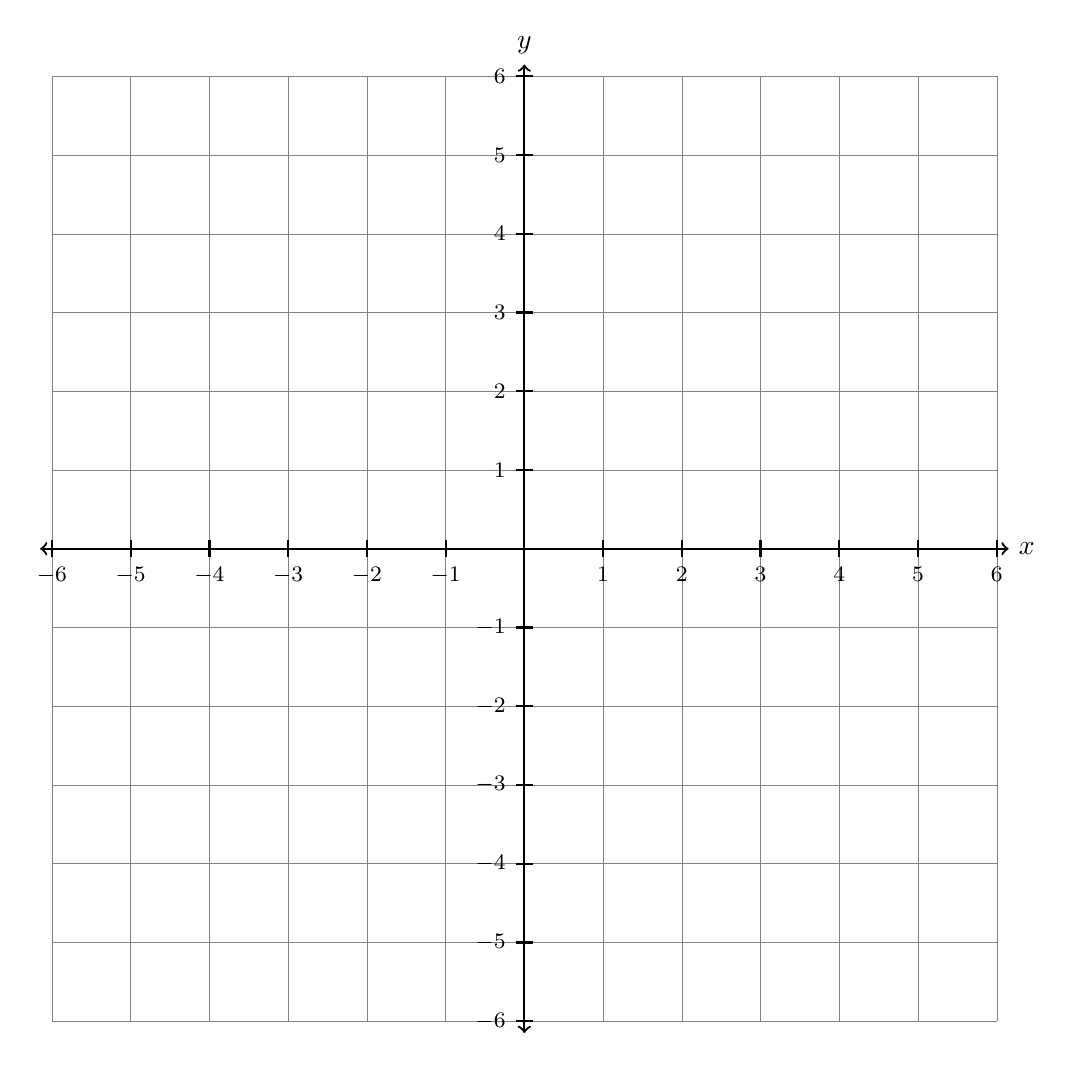
\begin{tikzpicture}

  % grid black help lines default colour is black!40
  \draw[help lines, step = 1cm] (-6, -6) grid (6, 6);

  % axis with end labels
  \draw[thick, <->] (0, -6.15) -- (0, 6.15) node[above] {$y$};
  \draw[thick, <->] (-6.15, 0) -- (6.15, 0) node[right] {$x$};

  % numbers along each axis .
  \foreach \x in {-6,-5,...,-1,1,2,...,6}
    \draw [thick] (\x cm,3pt) -- (\x cm,-3pt) node[anchor=north] {\fontsize{8}{11}\selectfont$\x$};
  \foreach \y in {-6,-5,...,-1,1,2,...,6}
    \draw [thick] (3pt,\y cm) -- (-3pt,\y cm) node[anchor=east] {\fontsize{8}{11}\selectfont$\y$};

\end{tikzpicture}
\end{document}